\section{Methodology: Extracting Mantle Library}

\begin{itemize}
  \item C bindings for Mantle
\end{itemize}

\subsection{Pluggable Interfaces}

\begin{figure}[tb]
  \noindent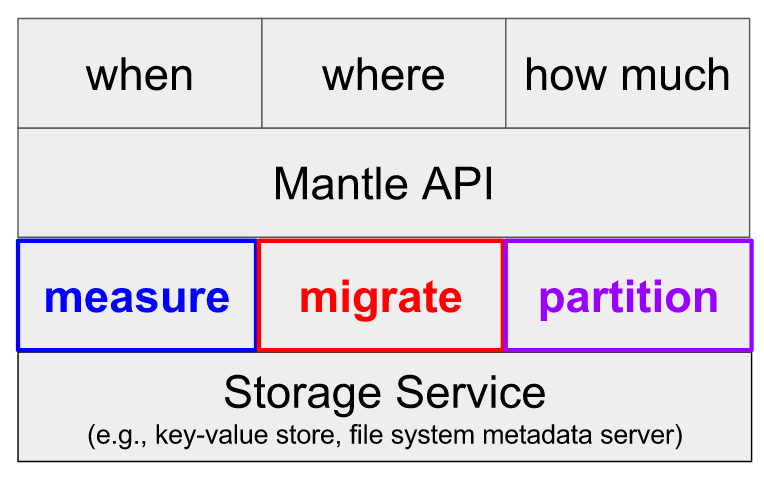
\includegraphics[width=19pc,angle=0]{figures/mantle-pluggable-interfaces.png}\\
  \caption{The storage service must: \textcolor{blue}{\textbf{measure}}
  resource usage, \textcolor{red}{\textbf{migrate}} resources, and
  \textcolor{purple}{\textbf{partition}} resources. }
  \label{fig:mantle-pluggable-interfaces}
\end{figure}

\subsubsection{Measure}

The metrics measured should help the system decide ``when" to migrate server
load. They should:

\begin{itemize}
  \item tell us about the state of the server or cluster
  \item provide some value of load, so we can partition/send it
\end{itemize}

In Ceph: global and local metrics ({\it e.g.}, CPU utilization, file system operation counts) \\

In HXHIM: ???\\

\subsubsection{Migrate}

In Ceph: \texttt{export\_dir()}

In HXHIM: \texttt{mdhimBPut()}, \texttt{mdhimBGet()}, ``adjusting ... keys" ???

\subsubsection{Partition}

In Ceph: subtrees and directory fragments

In HXHIM: secondary indices, cursor types, bul operations
